\newpage
\section{Le programme global des
\EUA}

\newthought{Le premier programme} connu pour avoir été massif dans ses
interceptions est ECHELON. Comme nous l'avons vu en introduction ce dernier fut
révélé en 1988 par un journaliste d'investigation spécialisé dans les services
de renseignements, mais son origine remonte jusqu'au traité UKUSA signé en 1946.
Les autres membres de Five Eyes ne rejoignirent ces deux pays qu'au cours des
années 1980, assurant ainsi une couverture globale des interceptions.

\begin{figure}
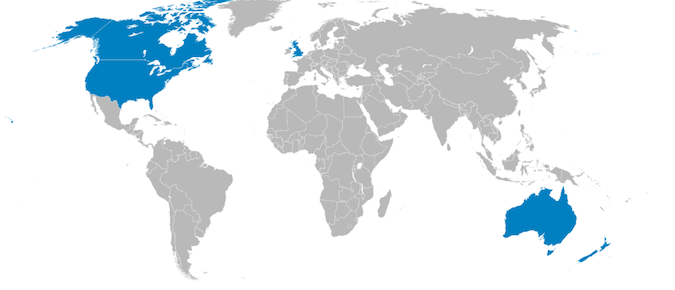
\includegraphics{fiveeyes.png}
\caption[Cartes de pays membres des Five Eyes][6pt]{Cartes de pays membres des
Fives eyes.}
\label{fig:carte}
\end{figure}

\newthought{Ce n'est qu'à} la fin des années 1960\autocite{ZDNET} qu'ECHELON fut
vraiment développé, lors des lancements des premiers satellites Intelsat. La
NSA\footnote{National Security Agency, l'agence chargée de la collecte des
informations électromagnétiques aux \EUA} et le GCHQ\footnote{Government
Communications Headquarters, le pendant britannique de la NSA} avaient besoin
d'accéder aux communications passées sur ces satellites, et décidèrent
donc de développer un réseau de stations d'écoutes terrestres, leur permettant
ainsi d'intercepter toutes les communications. Ainsi naquit ECHELON tel qu'on le
connaît encore aujourd'hui.

\newthought{Le programme s'est} renforcé au fur et à mesure des années, avec de
nouvelles stations, une orientation vers des interceptions sur fibre optique,
etc. Actuellement, il y aurait une quinzaine de stations d'écoutes réparties
dans le monde, selon un document de Snowden datant de 2012\autocite{Stations}.

\vspace{0.7cm}
\begin{figure}
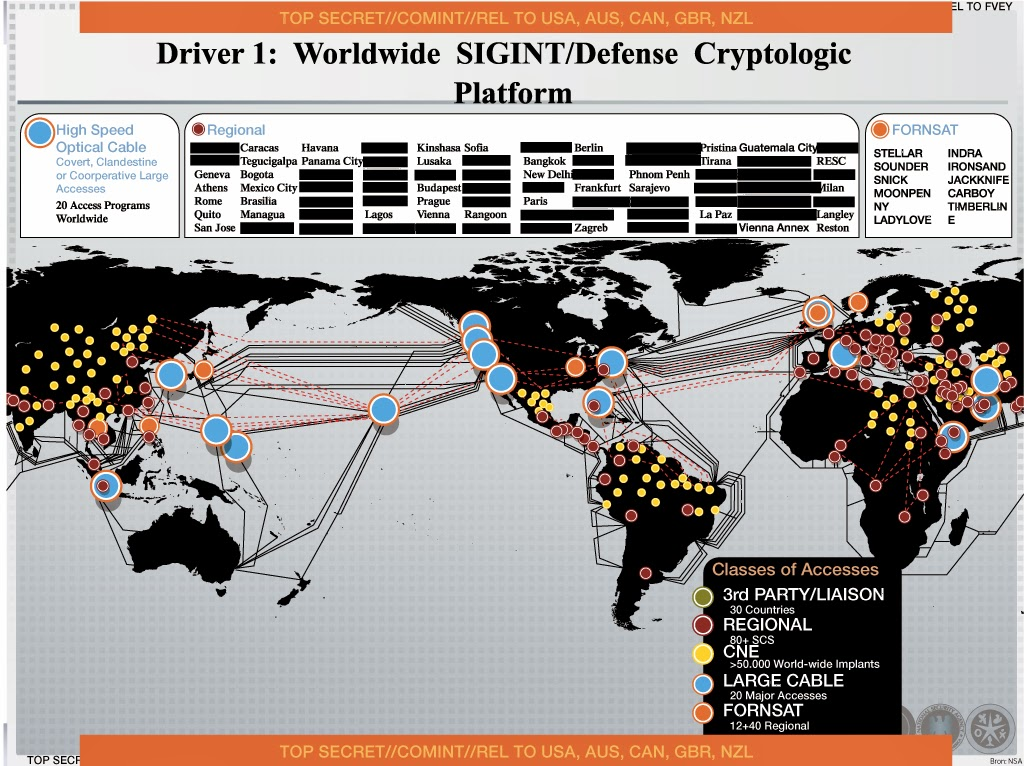
\includegraphics{carte.jpg}
\caption[Carte des stations d'interceptions][6pt]{Les points oranges
représentent les stations d'interceptions satellites.}
\label{fig:stations}
\end{figure}

\newthought{Comme le montre} la figure \ref{fig:stations}, les écoutes
concernent aussi maintenant les câbles sous-marins (contenant des fibres optiques) par
lesquels transitent 99\% des communications mondiales. 

\newthought{La NSA opère} également toute une myriade de programmes de
renseignement, afin de donner du sens aux données recueillies par les stations.
Du temps d'ECHELON, cela consistait en de gigantesques dictionnaires contenant
des mots-clés, que les supercalculateurs en charge de l'analyse pouvaient
isoler.

\newthought{Les documents de} Snowden ont permis de mettre à jour les détails
techniques des nouveaux programmes, dont les plus connus sont :

\subsection{PRISM}
\newthought{Le programme qui} a reçu le plus d'attention médiatique
lorsque les premiers documents de Snowden ont commencé à être révélés au public,
et certainement à juste titre, puisque le trafic généré par ce programme
représente 91\% du trafic de la NSA\autocite{WP91}. Les données proviennent
exclusivement des grandes entreprises du Web américaines (Google, Facebook,
Apple, etc) via l'utilisation de sélecteurs (des mots-clés, ou des requêtes
initiées par des analystes) qui vont aller chercher les informations quasiment
automatiquement.

\newthought{Ces révélations sur} les accès quasi-directs que possède la NSA sur
les serveurs des géants du Web furent très mal accueillies par ces derniers, qui
ont riposté en activant le chiffrement des communications sur leurs flux
internes\autocite{WPGoogle}, mettant à mal tout le dispositif clandestin. Il n'en
reste pas moins possible de passer par la voie légale pour obtenir les mêmes
données.

\newthought{En effet,} il est bon de rappeler brièvement que ces programmes ont
tous une base légale, à travers le FISA\footnote{Foreign Intelligence
Surveillance Act}. Ce texte, voté par le Congrès, décrit les modalités de
surveillance des citoyens \emph{étrangers}, impliquant que ces écoutes, ces
collectes et ces analyses en masse sont légalement permises. Elles n'ont pas
été remises en cause depuis l'instauration du Patriot Act en réaction aux attentats du 11 Septembre 2001.
Ce n'est que récemment (et suite aux révélations de Snowden) que ces programmes
et les pouvoirs qui leurs sont accordés furent remis en question.

\subsection{XKeyScore}
\newthought{L'un des programme} les plus mal connu, malgré les
documents publiés, mais également un des plus effrayants, de par l'ampleur de
son rayon d'action. 

\newthought{Il permettrait,} selon Glenn Greenwald, le journaliste qui a
interviewé Snowden et récupéré ses documents de <<~\ldots lire n'importe quel
courriel désiré, écouter n'importe quel appel téléphonique, historique de
navigation Web, documents Word. Et tout cela est fait sans demander à une cour,
sans demander l'approbation d'un superviseur pour cette part
d'analyse.~>>\autocite{GGW}

\newthought{Ce n'est pas} sans poser problème, puisqu'effectivement, ce dernier
ne semble pas avoir besoin de l'approbation de la FISC\footnote{Foreign
Intelligence Surveillance Court} pour les requêtes qui lui sont
fournies\autocite{Kimery}, contrairement au programme qui le précédait.

\subsection{Bullrun}

\newthought{C'est actuellement le} programme le plus cher de la NSA, avec un
coût total depuis son lancement, il y a dix ans, estimé à 800 millions
d'euros\autocite{bullrun} (par comparaison, PRISM ne coûte << que >> 20 millions
d'euros par an\ldots).
Sa fonctionnalité première semble être le décryptage de fichiers et de flux
chiffrés que l'Agence met de côté lorsqu'elle les intercepte. 

\newthought{Il semblerait aussi} qu'une autre facette de ce programme soit non
plus de l'ordre de la technique, mais dans la manipulation des standards de
chiffrement. En effet, il semble que la NSA ait poussé, au sein des instances
internationales en charge de la standardisation des méthodes de chiffrement, des
protocoles et des algorithmes qu'elle savait pouvoir casser\autocite{NYTenc} ou dans
lesquels elle avait délibérement inséré des portes dérobées.

\subsection{Dishfire}

\newthought{Ce programme est} actuellement opéré en partenariat avec le GCHQ
anglais. Il est spécialisé dans la collecte de messages textes (SMS) et dans la
géo-localisation de ces messages, la collecte de cartes de données
électroniques, des transactions de cartes de crédit circulant sans chiffrement sur le réseau,
les alertes d'appels manqués, les répondeurs, etc.

\newthought{Des aveux même} des analystes de la NSA et du GCHQ lors de la
présentation interne de ce programme, ce dernier collecte << à peu près tout ce
qu'il peut, donc vous pourriez voir des SMS de personnes qui ne sont pas visées
par vos requêtes. >>\autocite{Guardian}.

\newthought{Le gros avantage} de ce système est qu'il est possible de venir y
fouiller à posteriori. Lorsqu'une nouvelle cible est rentrée dans la base de
données, il est ainsi possible de retrouver ses anciens SMS et positions
géo-localisées afin d'affiner le profil.

\subsection{Upstream}

\newthought{Là où PRISM} pouvait être décrit comme << collecter tout ce qu'il
peut être collecté sur les réseaux sociaux >>, Upstream peut être décrit comme
<< collecter tout ce qu'on peut sur tout le reste >>. Contrairement à PRISM qui
est un programme autonome, Upstream se compose de multiples sous-programmes
(dont certains se composent eux-même de sous-programmes, il faut arriver à
suivre\ldots) :

\begin{itemize}
  \item FAIRVIEW : le programme chapeautant les trois autres.
  \item BLARNEY : se concentre sur la collecte de meta-données sur le réseau
  d'AT\&T\footnote{Grand opérateur de téléphonie américaine.}
  \item STORMBREW : se concentre sur les interceptions au niveau de l'opérateur
  Verizon.
  \item OAKSTAR : regroupement de 8 sous programmes, chacun spécialisé dans
  l'interception de méta-données dans une partie du monde.
\end{itemize}

\newthought{Selon les officiels}, cette collecte génère un flux très important
de données, et plusieurs filtres sont appliqués aux données collectées : les
opérateurs (AT\&T, Verizon, etc) font un premier filtre, en essayant de
supprimer au maximum les communications comprenant des citoyens américains.
Les communications restantes sont ensuite passées dans des sélecteurs (adresses
IP, numéros de téléphone, adresses mail, etc) afin d'en faire ressortir des
résultats. Le reste des données Internet peut ensuite être copié et utilisé à
travers XKeyScore pour des recherches futures.


\newthought{Tout ces programmes} ne sont que les plus gros exemples qui ont pu
être tirés des documents de Snowden. Il en existe encore beaucoup d'autres
(BoundLess Informant, RAGTIME, MAINWAY, MonsterMind, MYSTIC, TrailBlazer puis
Turbulence, MARINA, Dropmire pour les ambassades, Stateroom, etc), opérés par
la NSA seule ou bien en partenariat avec d'autres agences comme le GCHQ ou le
BND.

\vspace{0.8cm}
\begin{figure}
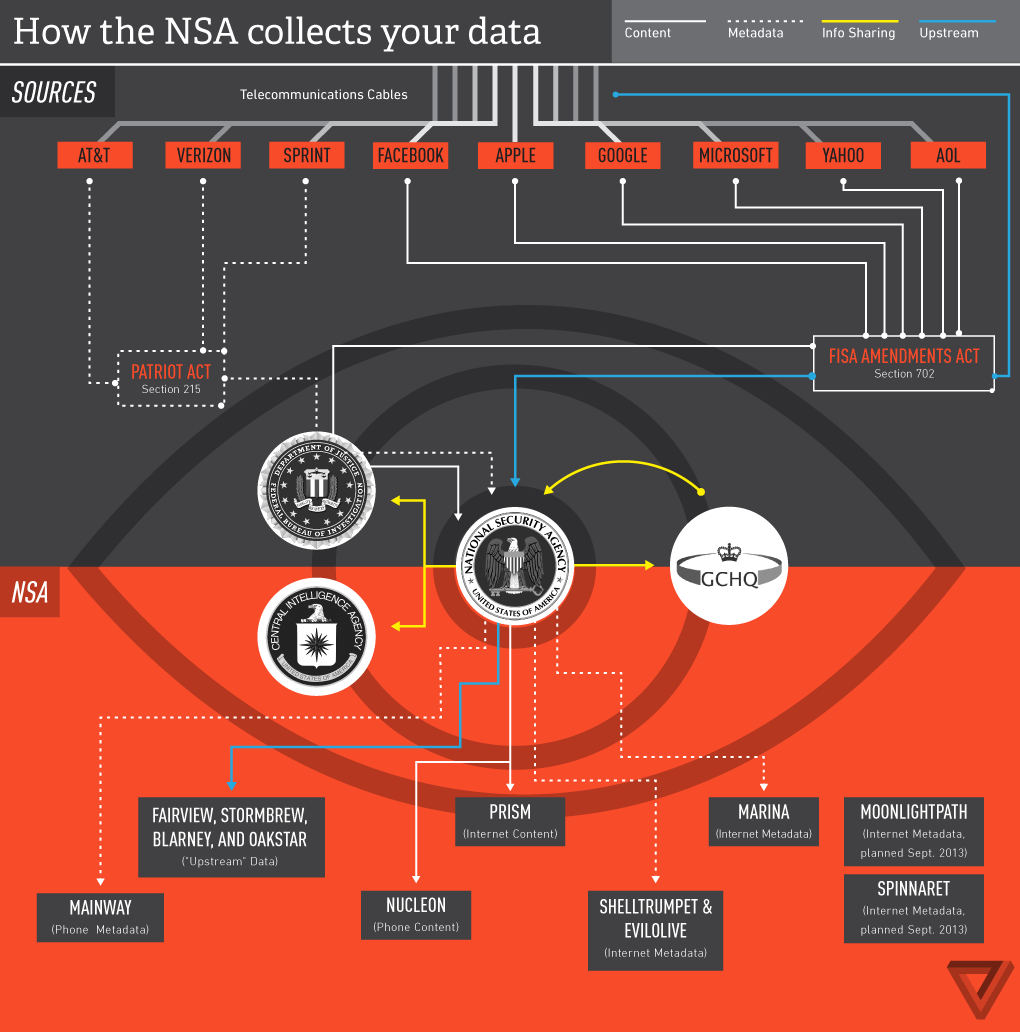
\includegraphics{flow.png}
\caption[Infographie résumant les différents programmes de
surveillance américains][6pt]{Résumé des différents programmes de collecte de
données de la NSA.}
\label{fig:infographie}
\end{figure}